\section{$MM^{2}$ resolution}
\label{Set: cut on MM}
\subsection{Control sample}

To study the resolution of $MM^{2}$, the control sample $e^{+} e^{-}
\rightarrow p \bar{p} K^{+} K^{-} \pi^{+} \pi^{-}$, and $D^{+}_{s}
\rightarrow K^{+} K^{-} \pi^{+},D^{-} _{s} \rightarrow K^{+} K^{-}
\pi^{-}$ are selected. The pion is the missing particle in those
sample. And the $MM^{2}$ is defined in Eq. \ref{Eq:def MM}.    

\begin{align}
    MM^{2} = \sqrt{ \left( E_{cm} - E_{p} - E_{\bar{p}} - E_{K^{+}} - E_{K^{-}} - E_{\pi} \right)^{2} - 
    \left( P_{p} + P_{\bar{p}} + P_{K^{+}} + P_{K^{-}} + P_{\pi} \right)^{2} } \\
    MM^{2} = \sqrt{ \left( E_{cm} - E_{K^{+}} - E_{K^{-}} - E_{K^{+}} - E_{K^{-}} - E_{\pi} \right)^{2} - 
    \left(  P_{K^{+}} + P_{K^{-}} + P_{K^{+}} + P_{K^{-}} + P_{\pi} \right)^{2} }
    \label{Eq:def MM}
\end{align}

And the event selection criteria is same as the detail listed in Sec.
\ref{Sec: PID} and Sec. \ref{Sec: General Event Selection}.

\subsection*{Compare Resolution between data and MC}
    
The difference of resolution between data and MC is defined in Eq.
\ref{Eq: delta resolution}.

\begin{equation}
    \Delta \sigma = \sqrt{ \sigma_{data}^{2} - \sigma_{MC}^{2} }
    \label{Eq: delta resolution}
\end{equation}
where $\sigma_{data}$ and $\sigma_{MC}$  are the resolutions of
$MM^{2}$ for data and MC sample, respectively.  The difference between
data and MC are listed in Tab. \ref{Tab: difference between data and
MC}. Where $\mu$ is the mean of $MM^{2}$, $\Delta \mu$ is the
difference of mean between data and MC, defined in Eq. \ref{Eq:
difference of mean}.

\begin{equation}
    \Delta \mu = \mu_{data} - \mu_{MC}
    \label{Eq: difference of mean}
\end{equation}

\begin{table}[htbp]
    \caption{Difference between data and MC.}
    \label{Tab: difference between data and MC}
    \scalebox{0.7}{
        \begin{tabular}{l|ccc|ccc}
            \hline \hline
            Sample     &    $\sigma_{data} (GeV^{2}/c^{4})$   & $\sigma_{MC} (GeV^{2}/c^{4})$ 
            & $\Delta \sigma (GeV^{2}/c^{4})$ & $\mu_{data} (GeV^{2}/c^{4}) $ & $\mu_{MC} (GeV^{2}/c^{4}) $ & $\Delta \mu (GeV^{2}/c^{4})$ 
            \\ \hline 
            $e^{+} e^{-} \rightarrow p \bar{p} K^{+} K^{-} \pi^{+} \pi^{-}$    & $0.0089 \pm 0.0002$ & $0.0091 \pm 0.0001$ &
            $-0.0001 \pm 0.0002$ & $0.02011 \pm 0.0003$ & $0.0199 \pm 0.0000$ & $0.0002 \pm 0.0003$ 
            \\ \hline  
            $D^{+}_{s} \rightarrow K^{+} K^{-} \pi^{+},D^{-} _{s} \rightarrow K^{+} K^{-} \pi^{-}$ 
            &  $0.1227 \pm 0.0002$ & $ 0.1241 \pm 0.0013 $   & $0.0014 \pm 0.0013 $ & $0.2118 \pm 0.0018 $ 
            & $ 0.2070 \pm 0.0003 $ & $ 0.0048 \pm 0.0019$
            \\ \hline
            \hline

        \end{tabular}
    }
\end{table}

We find the relative change of mean and resolution are consisted for
those two control sample as listed in Tab. \ref{Tab: relative change of
sigma}. So we take the relative change of mean and resolution to modify
the $MM^{2}$ to obtain the systematic uncertainty. It's reasonable to
obtain the difference of mean and resolution: 

\begin{equation}
    \frac{\Delta \sigma}{\sigma_{data}} = 1.2 \pm 1.1 \%,~\frac{\Delta \mu}{\mu_{data}}= 2.3 \pm 0.9 \%
    \label{Eq: result of dSigma}
\end{equation}
    
\begin{table}[htbp]
        \caption{The relative change of mean and resolution for data and MC}
        \label{Tab: relative change of sigma}
        \centering
     \scalebox{1.0}{
        \begin{tabular}{lcc}
        \hline \hline
        Sample     &    $ \frac{\Delta \sigma}{\sigma_{data}} (\%)$   & $\frac{\Delta \mu}{\mu_{data}}  (\%)$  \\ \hline
         
        $e^{+} e^{-} \rightarrow p \bar{p} K^{+} K^{-} \pi^{+} \pi^{-}$    & $ -1.1 \pm 2.1$  & $ 1.0 \pm 1.5$ \\ \hline
       
        $D^{+}_{s} \rightarrow K^{+} K^{-} \pi^{+},D^{-} _{s} \rightarrow K^{+} K^{-} \pi^{-}$ & $ 1.2 \pm 1.1$ & $ 2.3 \pm 0.9 $  
        \\ \hline
        \hline
        
        \end{tabular}
    }
\end{table}

The correction is perform in such process,  Smear the MC sample with a
Gaussian function with standard deviation and the central value
determined according to Eq. \ref{Eq: result of dSigma}. And the
standard deviation of the Gaussian function is taken as the difference
of resolution between data and MC, i.e. the $\Delta \sigma$ in Tab.
\ref{Tab: relative change of sigma}, so as the mean of the Gaussian
function.  We change the tandard deviation and the central value of the
Gaussian function, obtain the biggest relative change is 0.95\%. So we
set the systematic uncertainty at 1\%.
    
\begin{figure}[htbp]
    \centering
    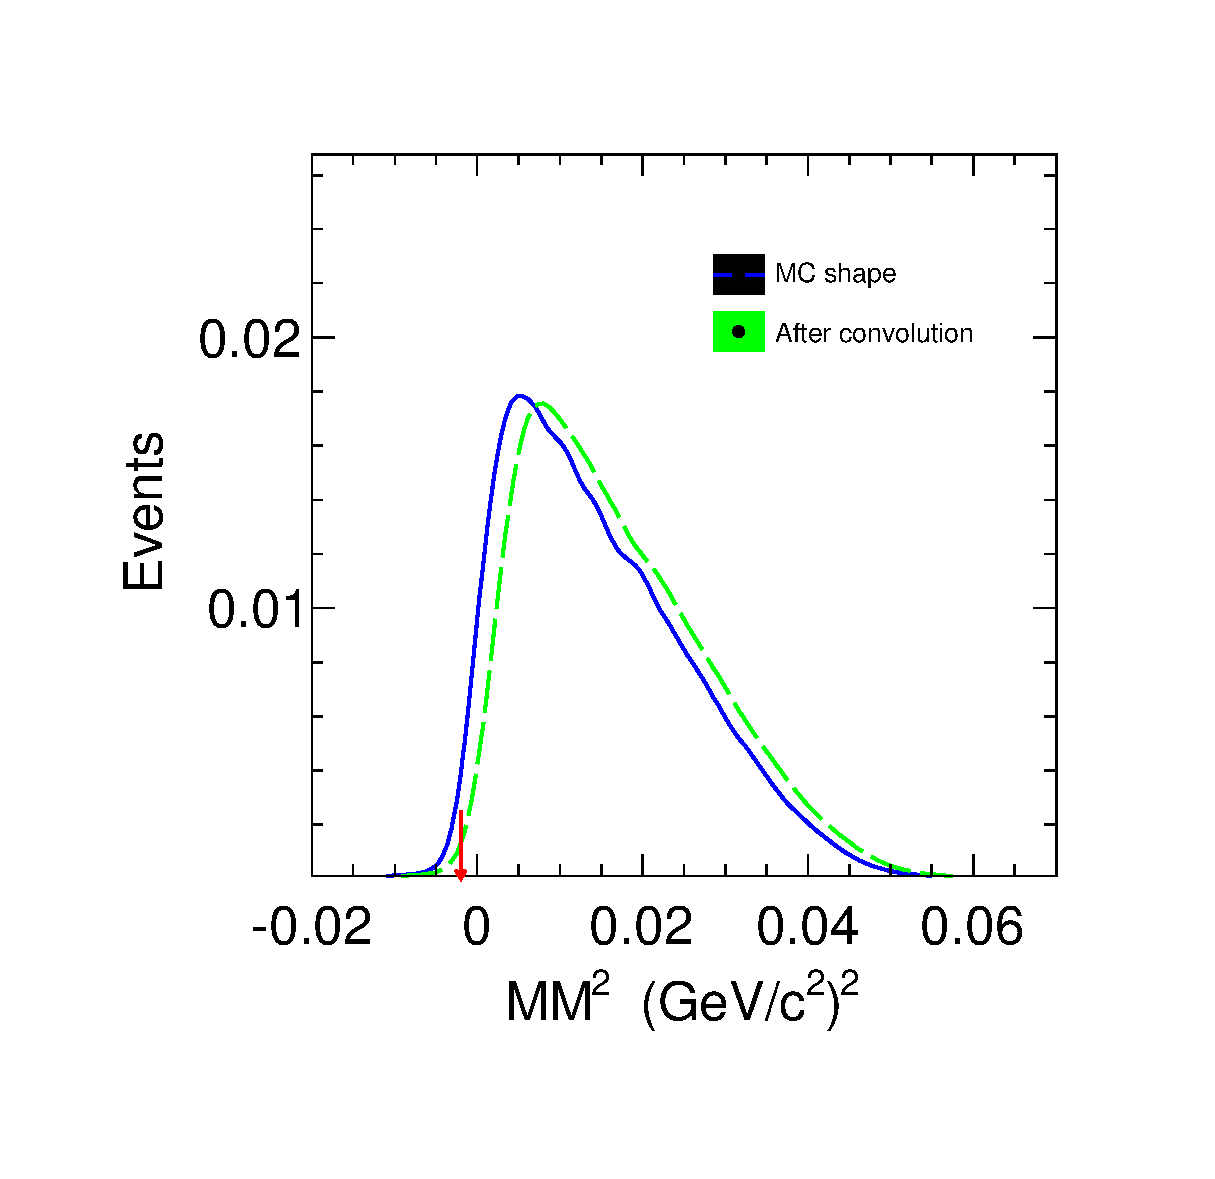
\includegraphics[width = 8 cm]{section/append/fig/Cov_MM.eps}
    \caption{The distribution of $MM^{2}$ after convoluted with a Gaussian function. The arrows show the requirement on $MM^{2}$ for data and MC.}
    \label{Fig: Covolution gaussian}
\end{figure}

